\section{Dimensionierung des Baluns}

Wie im Abschnitt \ref{sec:strombalun} ersichtlich ist, hat ein Strombalun einige Vorteile gegenüber dem Spannungsbalun. Da vor allem die Anforderungen an den Kern kleiner sind und damit die Dimensionierung vereinfacht wird, haben wir uns für einen Strombalun entschieden. Da beim klassischen Strombalun keine Impedanzanpassung geschieht, diese jedoch für unsere Anwendung gewünscht wird, verwenden wir einen Guanella-Balun. Der Guanella-Balun ist ein Spezialfall, bei dem mehrere klassiche Strombaluns zusammengschaltet werden, so dass das Impedanzverhältnis von Ein-zu Ausgang der folgenden Formel entspricht:
Dabei entspricht n der Anzahl klassicher Balunstufen.

\begin{equation}
	\frac{Z_{out}}{Z_{in}}=n^{2} \hspace{1cm} n\in\mathrm{N}
\end{equation}

Um unsere 200$\Omega$-Dipol-Antenne an das 50$\Omega$-Koaxialkabel anzupassen benötigen wir dementsprechend einen Guanella-Balun mit zwei Stufen. Daraus resultiert ein Impedanzverhältnis von \(1:4\).

\subsection{Ersatzschaltung}
Bei nachfolgender Betrachtung beschränken wir uns auf den klassischen Strombalun. Damit werden die Berechnungen (wie z.B. die Resonanzfrequenz) stark vereinfacht und können später auf den Guanella-Balun übertragen werden. In Abbildungn \ref{fig:ersatz_spule} ist das Ersatzschaltbild einer realen Spule ersichtlich. Dies besteht aus einer idealen induktivität $L$, aus zwei Widerständen, welche die Magnetisierungs- ($R_{fe}$) und Kupferverluste ($R_{cu}$) modelieren und einer parallelen Kapazität $C_{p}$ für die Kapazität zwischen den einzelnen Windungen.

\begin{figure}[H]
	\centering
	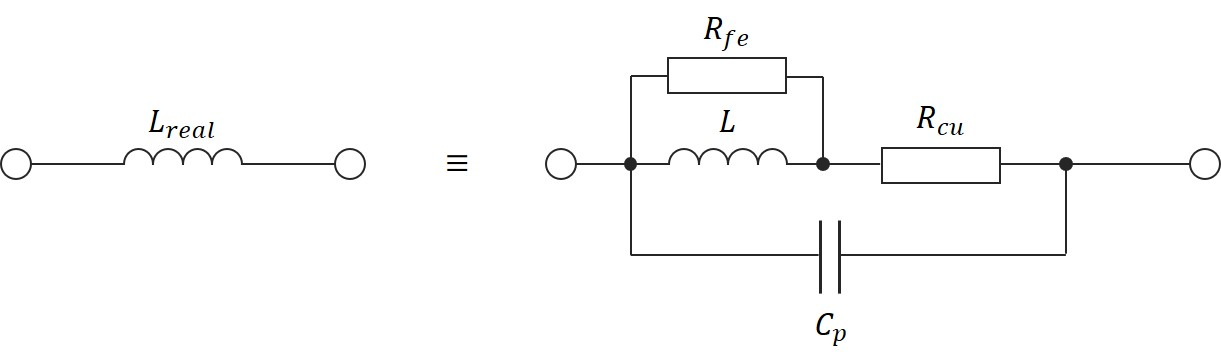
\includegraphics[width=0.7\linewidth]{Ersatzschaltung_Spule.jpg}
	\caption{Ersatzschaltung einer realen Spule}\label{fig:ersatz_spule}
\end{figure}

Die Abbildung \ref{fig:klassischer_strombalun} zeigt den einfachen Strombalun. Die Induktivitäten können seriell betrachtet werden, was die nachfolgenden Berechnungen vereinfacht. Bei der Dimensionierung des Baluns, wird der Lastwiderstand $R_{L}$ vernachlässigt und nur die Impedanz des Baluns ($2\cdot L'$ in Serie) untersucht. Ist diese Impedanz viel grösser als der Lastwiderstand ($\gg \SI{200}{\Omega}$), so sperrt der Balun, was für Gleichtaktströme gewünscht wird. Ist die Impedanz kleiner als der Lastwiderstand ($\ll \SI{200}{\Omega}$), so  wird das Signal durchgelassen. Dies wird im Gegentaktmodus angestrebt.

\begin{figure}[H]
	\centering
	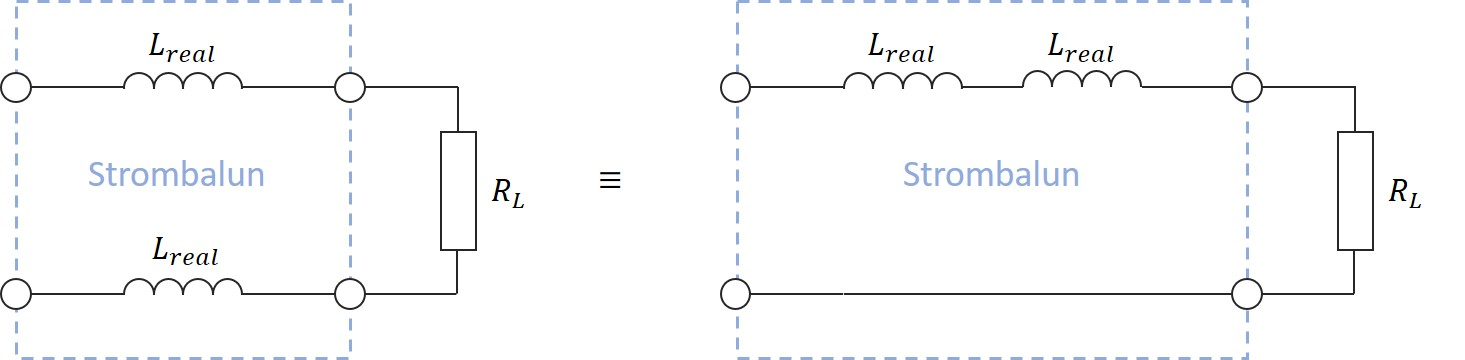
\includegraphics[width=0.7\linewidth]{Klassischer_Strombalun.jpg}
	\caption{Einfacher Strombalun}\label{fig:klassischer_strombalun}
\end{figure}



\newpage

Um das Verhalten eines Baluns zu beschreiben, macht es Sinn, zwischen Gleich- und Gegentaktmodi zu unterscheiden. Wir versuchen nun unseren Balun so zu dimensionieren, damit er bei der gewählten Arbeitsfrequenz von \SI{20}{MHz} im Gleichtaktmodus sperrt, und im Gegentatkmodus leitet. Können wir dies gewährleisten, haben wir keine störenden Mantelwellen auf dem Koaxialkabel.

\paragraph{Gegentaktbetrieb}
In Abbildung \ref{fig:diff_mode} ist ein vereinfachtes Ersatzschaltbild für den Gegentaktbetrieb ersichtlich. Dies hat Gültigkeit unter der Annahme, dass sich die Felder der beiden Spulen komplett aufheben. In diesem Fall kann man die Spulen als Kurzschluss und die Magnetisierungsverluste als Unterbruch betrachten. 
Weil der Kupferwiderstand viel kleiner als der Lastwiderstand ist und somit gilt:  $R_{cu} \ll R_{L}$, passieren Gegentaktströme praktisch ungehindert den Balun.
\begin{figure}[H]
	\centering
	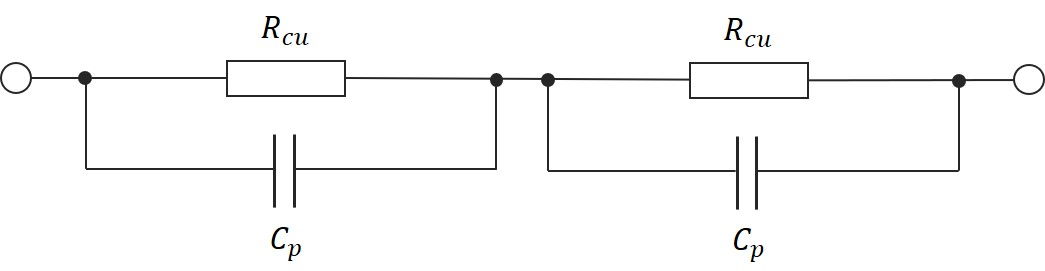
\includegraphics[width=0.8\linewidth]{diff_mode.jpg}
	\caption{Situation im Gegentaktbetrieb}\label{fig:diff_mode}
\end{figure}

\paragraph{Gleichtaktbetrieb}
In Abbildung \ref{fig:com_mode} ist ein vereinfachtes Ersatzschaltbild für den Gleichtatkbetrieb dargestellt. In diesem Fall kann der Kupferwiderstand vernachlässigt werden. Die beiden Parallelschwingkreise, welche in Serie geschaltet sind, können zu einem einzelnen Parallelschwingkreis zusammengefasst werden. Da unser Ziel darin besteht, eine möglichst hohe Impedanz zu erreichen, wird dieser der Balun so dimensioniert, dass die Resonanzfrequenz im Arbeitspunkt zu liegen kommt. Aus den Grundformeln des Parallelschwingkreises, lassen sich folgende Formeln für den Balun ableiten. \cite{balun_schneider}

\begin{equation}
\omega_{0} = \frac{1}{\sqrt{L \cdot C_{p}}}
\label{equ:Resonanzfrequenz}
\end{equation}

\begin{equation}
Q = 2 \cdot R_{FE} \cdot \sqrt{\frac{C_{p}}{4 \cdot L}}
\label{equ:Güte}
\end{equation}

\begin{figure}[H]
	\centering
	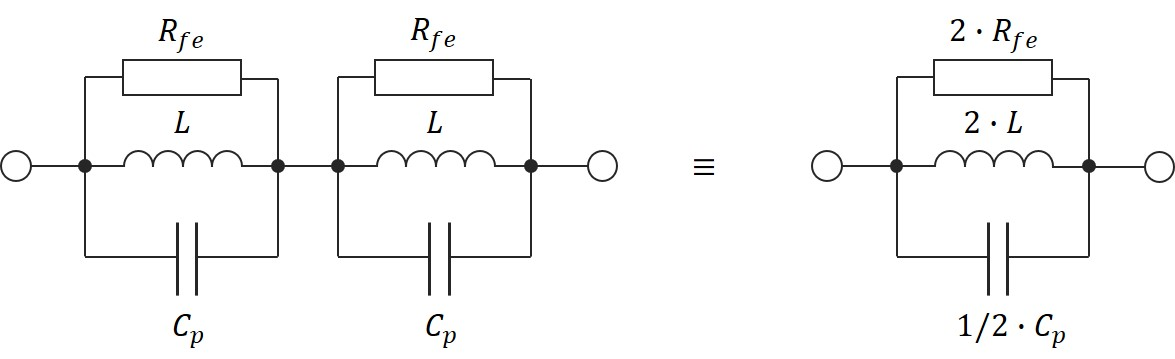
\includegraphics[width=0.8\linewidth]{com_mode.jpg}
	\caption{Situation im Gleichtaktbetrieb}\label{fig:com_mode}
\end{figure}

\subsection{Die Kernfrage}
Damit sich die Felder im Gegentaktmodus aufheben, muss ein Kern mit hoher Permeabilität verwendet werden. Dadurch wird ein höherer Kopplungsfaktor zwischen den Spulen ermöglicht und gleichzeitig kann eine höhere Induktivität bei gleicher Windungszahl erreicht werden. In der Formel \ref{equ:Güte} ist ersichtlich, dass die Güte des Schwingkreises umgekehrt proportional zu den Magnetisierungsverlusten $R_{FE}$  bei der Resonanzfrequenz ist. Verwendet man einen Kern mit hohen Magnetisierungsverlusten, wird der Balun breitbandiger, sperrt jedoch unerwünschte Mantelwellen weniger. Verwendet man einen Kern mit wenigen Verlusten, ist das Gegenteil der Fall.
Für unsere Anwendung ist kein breitbandiger Balun gefordert, aber um das Wickeln der Spulen zu vereinfachen, verwenden wir einen eher breitbandigen Kern. Dies gibt uns einen Spielraum bei der Realisierung. Deshalb verwenden wir anstelle eines Eisenkerns einen Ferritkern. (Ersterer ermöglicht eine hohe Güte, bei geringer Bandbreite.)

%Hier Bild 

Wir haben mit folgenden Kriterien nach einem Ferrit gesucht:
\begin{itemize}
	\item Form: Toroid
	\item Material: Ferrit
	\item Permeabilität: möglichst hoch bei 20MHz und wenn möglich konstant
\end{itemize}

Weil der Werkstoff 4C65 gemäss Abbildung \ref{fig:ferrit_kurve} bei 20MHz die höchste Permeabilität aufweist und diese auch ziemlich konstant ist, fiel die Wahl auf diesen Werkstoff.

\begin{figure}[H]
	\centering
	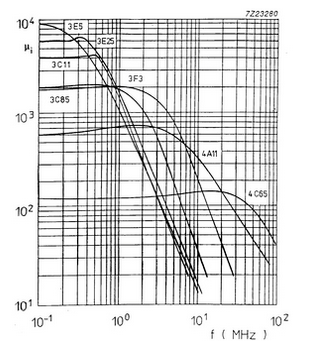
\includegraphics[width=0.7\linewidth]{ferrit_kurve.png}
	\caption{Permeabilität in Abhängigkeit der Frequenz verschiedener Werkstoffe}\label{fig:ferrit_kurve}
\end{figure}

\subsection{Windungszahl}
Da der Kern nun bestimmt ist, gilt es die Windungszahl zu bestimmen. Mit der Anzahl Windungen soll die Resonanzfrequenz auf unsere Arbeitsfrequenz abgestimmt werden. Wie bereits erwähnt, ist die Resonanzfrequenz folgendermassen definiert:
\begin{equation}
\omega_{0} = \frac{1}{\sqrt{L \cdot C_{p}}}
\label{equ:Resonanzfrequenz2}
\end{equation}

Die Induktivität einer Toroidspule kann mit folgender Formel berechnet werden. Dabei ist $N$ die Windungszahl, $b$ die Höhe des Toroids, $r_{2}$ der Aussendurchmesser und $r_{1}$ der Innendurchmesser des Toroids.
\begin{equation}
L_{Toroid} = N^{2}\cdot \frac{\mu_{0}\cdot \mu_{r}\cdot b}{2\cdot \pi}\cdot \ln \Big(\frac{r_{2}}{r_{1}}\Big)
\label{equ:L_Toroid}
\end{equation}

\begin{figure}[H]
	\centering
	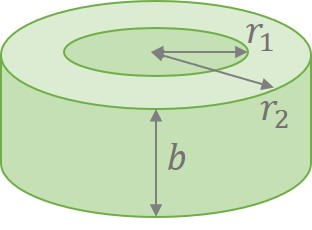
\includegraphics[width=0.3\linewidth]{Induktivitaet_Toroid.jpg}
	\caption{Geometrie Toroid}\label{fig:ind_toroid}
\end{figure}

Für die Eigenkapazität $C_{p}$ der Spule gibt es keine Eindeutige Formel. Wir haben deshalb versucht, diese mit starken Vereinfachungen zu berechnen. Dabei haben wir die runden Oberfläche zweier verdrillter Drähte als Plattenkondensatoren approximiert. Mit dem Korrekturfaktor $K1$ wird der Drahtdurchmesser auf die Plattenoberfläche abgebildet. Weil zwei Drähte nicht ideal aneinanderliegen, ist der Plattenabstand grösser als $2\cdot d_{I}$. Um dem gerecht zu werden, wurde der Korrekturfaktor $K2$ eingeführt. Die dabei entstandene Formel ist nachfolgen ersichtlich. Dabei ist $b$ wieder die Höhe des Toroids, $N$ die Windungszahl, $r_{cu}$ der Drahtradius und $d_{I}$ die Isolationsdicke.
\vspace{1cm}
\begin{equation}
C_{Toroid} = \varepsilon\cdot 2\pi\cdot b\cdot N\cdot \frac{r_{cu}\cdot K_{1}}{d_{I}\cdot 2\cdot K_{2}}
\label{equ:C_Toroid}
\end{equation}


\begin{figure}[H]
	\centering
	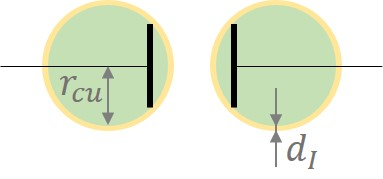
\includegraphics[width=0.5\linewidth]{Kapazitaet_Toroid.jpg}
	\caption{Vereinfachte Kapazität zweier benachbarter Windungen}\label{fig:cap_toroid}
\end{figure}

Substituiert man \ref{equ:C_Toroid} und \ref{equ:L_Toroid} in Formel \ref{equ:Resonanzfrequenz2} und löst nach der Windungszahl $N$ auf, erhält man schliesslich folgende Formel:

\begin{equation}
N = \sqrt[3]{\frac{2\cdot d_{I}\cdot K_{2}}{\omega_{0}^{2}\cdot \mu_{0}\cdot \mu_{r}\cdot \varepsilon_{0}\cdot \varepsilon_{r}\cdot b^{2}\cdot \ln \Big(\frac{r_{2}}{r_{1}}\Big)\cdot K_{1}\cdot r_{cu}}}
\label{equ:N_Toroid}
\end{equation}

\begin{table}[H]
	\centering
	\begin{tabular}{|l|l|l|ll}
		\cline{1-3}
		\textbf{Variable} & \textbf{Wert} & \textbf{Typ} &  &  \\ \cline{1-3}
	$\omega_{0}$	&   $2\pi\cdot 20MHz$        &     Aufgabenstellung      &  &  \\ \cline{1-3}
	$\mu_{0}$	&     $4\pi\cdot 10^{-7} N/A^{2}$      &  Konstante         &  &  \\ \cline{1-3}
	$\varepsilon_{0}$	&  $8.854\cdot 10^{-12} As/Vm $         &     Konstante      &  &  \\ \cline{1-3}
	$d_{I}$	&  $\SI{50}{\mu m}$         &     Datenblatt      &  &  \\ \cline{1-3}
	$\mu_{r}$	&  $150$         &     Datenblatt      &  &  \\ \cline{1-3}
	$\varepsilon_{r}$	&  $2.2$         &     Datenblatt      &  &  \\ \cline{1-3}
	$b$	&  $\SI{5.3}{mm}$         &     Datenblatt      &  &  \\ \cline{1-3}
	$r_{cu}$	&  $\SI{250}{\mu m}$         &     Datenblatt      &  &  \\ \cline{1-3}
	$r_{1}$	&  $\SI{13.1}{mm}$         &     Datenblatt      &  &  \\ \cline{1-3}
	$r_{2}$	&  $\SI{23.7}{mm}$         &     Datenblatt      &  &  \\ \cline{1-3}
	$K_{1}$	&  $1.5$         &     Geschätzt      &  &  \\ \cline{1-3}
	$K_{2}$	&  $3$         &     Geschätzt      &  &  \\ \cline{1-3}
	\end{tabular}
\end{table}

Eingesetzt in Formel \ref{equ:N_Toroid} resultiert eine Windungszahl $N$ von: $9.39$ Windungen.

\subsection{Draht oder Litze?}
Grundsätzlich wäre für beste Resultate Litze zu verwenden, um den Skin-Effekt zu minimieren. Dafür müsste spezielle HF-Litze verwendet werden. Bei dieser müssten die Leiter zueinander isoliert sein und im Mittel über den Querschnitt gleich verteilt sein. Da auch mit dem Skin-Effekt der Kupferwiderstand im Gleichtaktmodus vernachlässigt werden kann und im Gegentaktmodus bei hohen Frequenzen $C_{p}$ dominiert, können wir hier Draht verwenden.





